\section{Evaluation}
\label{sec:eval}
%
\begin{figure}[t!]
\begin{center}
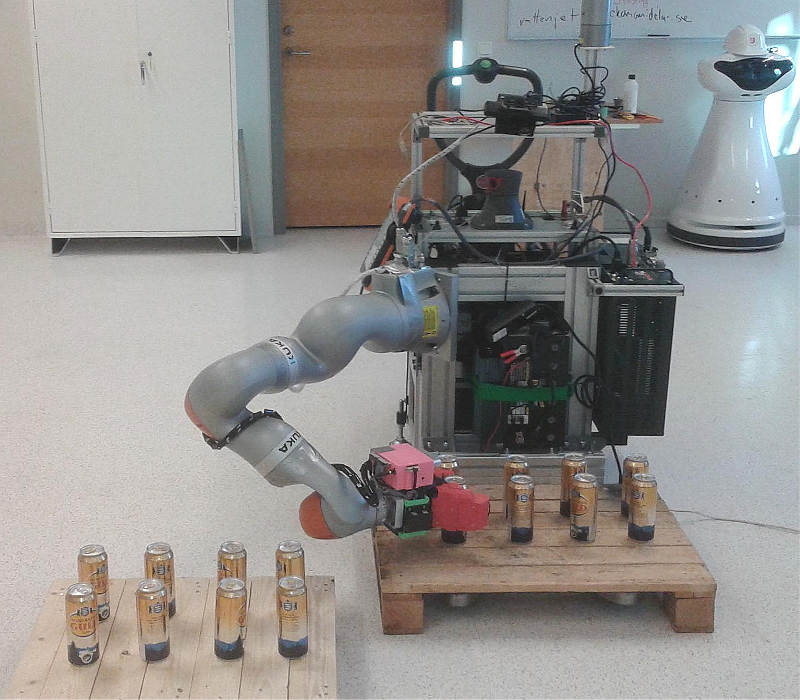
\includegraphics[width =1\linewidth]{figs/demo}
%\vspace{-0.25cm}
\caption{\textit{Demo setup:} The robot loads beer onto a previously picked up pallet and
  subsequently transports it to a predefined target location.}
\label{fig:demo_setup}
\vspace{-0.65cm}
\end{center}
\end{figure}
%


commands while accounting for the robot dynamics~\cite{Saab13})

The aim is to reduce the dependence on classical, sampling based motion planning and to move towards
reactive feedback control to generate and execute complex motion behaviors of a robot.  Here, only
high-level behavioral goals (e. g., “go to this region” or “stay above obstacle plane”) are
specified in form of task functions~\cite{Sams91}. An intelligent control algorithm, which is based
on embedded optimization of these task functions, then handles the details and synthesizes
appropriate motions automatically in an online fashion. Opposed to classical sense-plan-act
architectures, in this paradigm only task-relevant Degrees of Freedom (DoF) need to be constrained,
which allows to exploit kinematic redundancies, e. g., for a manipulator to avoid unexpected
obstacles. Regarding grasp planning, we follow the general tenet and will extract redundant
representations in form of constrained pose intervals instead of discrete poses


\cite{Kano09} task function description
\cite{Guro15}(Used off-the-shelf solver)
\cite{Quig09}(ROS)